\documentclass[thesis.tex]{subfiles}

\begin{document}
\subsection{Dark Matter} \label{subsec:DM}
\begin{figure}[t]
	\centering
	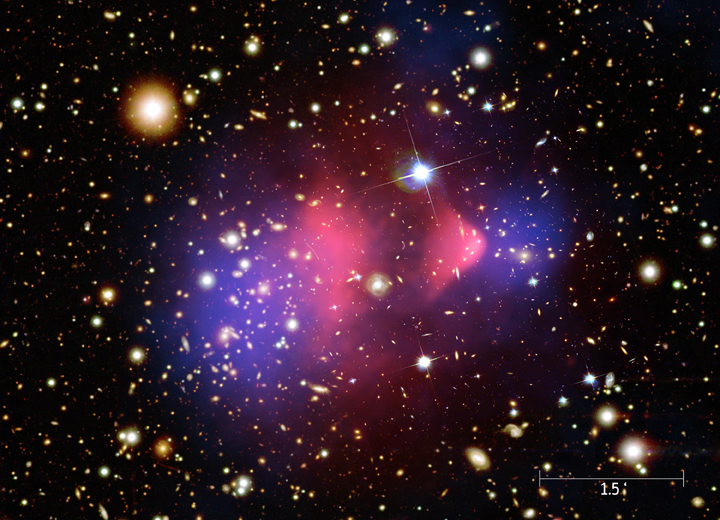
\includegraphics[width=0.8\linewidth]{figures/bullet-cluster.jpg}
	\caption{
	Composite image of the Bullet Cluster that shows the presence of dark matter through gravitational lensing.
	Pink regions are the X-rays of baryonic matter.
	Blue regions are from the gravitational lensing map.
	The scale on the bottom right is in arcminutes. \cite{Bullet-Image}
	}
	\label{fig:bullet-cluster}
\end{figure}
The effects of dark matter are apparent through various observations, such as the gravitational lensing within the Bullet Cluster \cite{Bullet}.
This cluster is the result of the collision between two galaxy clusters.
The baryonic matter is visible through X-ray images and acts as we'd expect: there is a drag between the two clusters that resulted in the Bullet Cluster's distinct shape \cite{Bullet}.
However, the massive portions of these clusters continue to move past each other as shown by the gravitational lensing map in Figure \ref{fig:bullet-cluster}.
These results are indicative of both the ``dark'' and weakly interacting nature of dark matter.
The particles are not visible through electromagnetism, thus receiving the name dark matter.
The particles have a mass that causes the gravitational lensing.
This upper limit on the related mass and collision cross section is given by Markevitch et al. \cite{Bullet} as:
\begin{equation} \label{eq:DM-Mass-Lim}
	\frac{\sigma}{m} < 1 \; \text{cm}^2 \text{g}^{-1}
\end{equation}
where $\sigma$ is the collision cross section and $m$ is the particle mass \cite{Bullet}.
A more detailed explanation of how this limit is derived can viewed in \cite{Bullet}.

\par One candidate for dark matter particles is the weakly interacting massive particle (WIMP) \cite{DM_Hist}.
This particle interacts by the electroweak force and has a lower bound of mass at the keV level \cite{DM_Hist}.
Thereby, a direct detection experiment must be sensitive to nuclear recoils at the keV level.
The XENON Collaboration produced the XENON1T detector for this exact purpose.
The collaboration has since built and started commissioning the successor XENONnT, but the topics discussed in this paper will be with regard to XENON1T.

\subsection{XENON1T Detector}\label{subsec:Xe1T}
\begin{figure}[t]
	\centering
	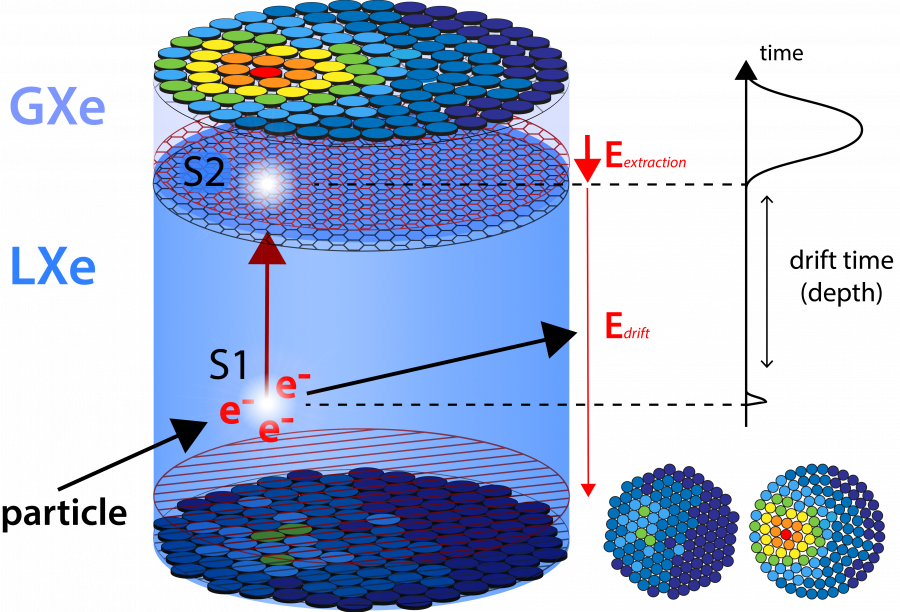
\includegraphics[width=0.8\linewidth]{figures/Xe1T-TPC.png}
	\caption{
	Diagram of the XENON1T detector and event scintillation and ionization.
	The first signal is the S1 where electrons and photons are emitted by the particle interaction.
	The electrons from the S1 are drifted upward by a constant electric field and extracted from the liquid phase to the gas phase using a stronger electric field.
	This produces the second signal S2 where more photons are emitted.
	The plane of circles at the bottom and top of the detector represent the photomultiplier tubes in the detector.
	The color of these circles indicate the photoelectrons observed for an S1 or S2 and is shown more clearly in Figure \ref{fig:example_hit}. \cite{Xe1T-Diagram}
	}
	\label{fig:Xe1T-TPC}
\end{figure}
The XENON1T detector is a dual phase xenon time projection chamber (TPC) located in the \textit{Laboratori Nazionali del Gran Sasso} (LNGS) in central Italy.
As stated in Sec. \ref{subsec:DM}, it was a requirement for the detector to be sensitive to keV energy levels in order to detect WIMPs.
To meet these requirements, the detector's placement in LNGS, use of xenon, and water shielding all serve to reduce the presence of extraneous signals that would be appear from muons and more radioactive media \cite{Xenon1t}.
It contains a target of $\sim$1.3 tons of liquid xenon and a fiducial volume with a maximum radius of 42.84 cm \cite{1TDM_DataAnalysis}.
The detector features 258 photomultiplier tubes (PMTs): 127 on the top array and 121 on the bottom array.
Over the course of the experiment, these PMTs will break and the signal they would see can no longer be used.
\begin{wrapfigure}{r}{0.5\textwidth}
	\centering
	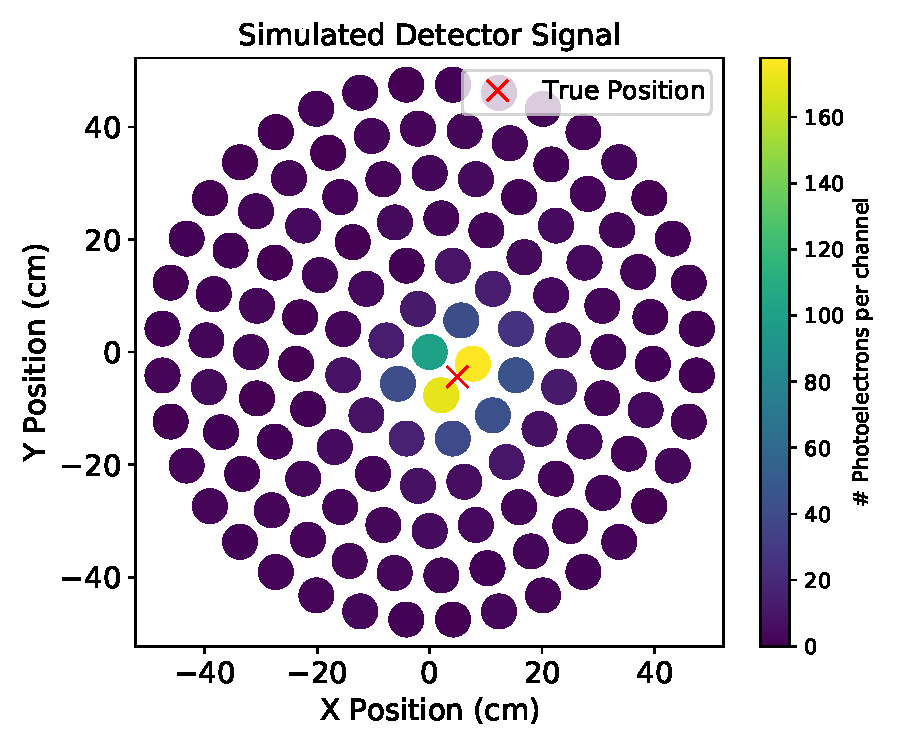
\includegraphics[width=\linewidth]{figures/opt_sim_hit_989.pdf}
	\caption{Example simulated hit pattern.
	Each circle represents a PMT in the top array of the detector.
	The position of each circle is the real position of the PMT in the detector.
	The simulation has a true position marked by the red x and created the shown hit pattern.}
	\label{fig:example_hit}
\end{wrapfigure}
\pdfmarkupcomment[markup=Highlight, color=yellow]{There is a constant electric field of 116.7 V/cm that causes electrons to drift towards the liquid-gas interface at the top of the detector, where they are extracted by a stronger electric field and produces a proportional scintillation signal}{Feels very awkward. Also seems close to the introduction of the citation.} \cite{Xenon1t}.

\par An event in the detector is defined by a particle scattering off xenon atoms.
The recoiling nuclei of the xenon atoms results in a scintillation and ionization.
The scintillation is observed by the PMTs and regarded as the S1 signal.
The signal produced by the ionization at the liquid-gas interface is regarded as the S2 signal.
An example of this signal is shown in Figure \ref{fig:example_hit}.
A diagram of the detector, S1, and S2 are shown in Figure \ref{fig:Xe1T-TPC}.
The resulting light pattern from the S2 signal is the observation that is used for our inverse problem.
The inverse problem exactly is to use this light pattern from the top array of PMTs to reconstruct the $(x, y)$ position of the event in reference to the plane of the PMTs.
It is unnecessary to include the depth, or $z$ position, of the event as that is achieved using the time separating the S1 and S2 and the known applied electric field.
This is the problem for position reconstruction.

\begin{figure}[t]
	\centering
	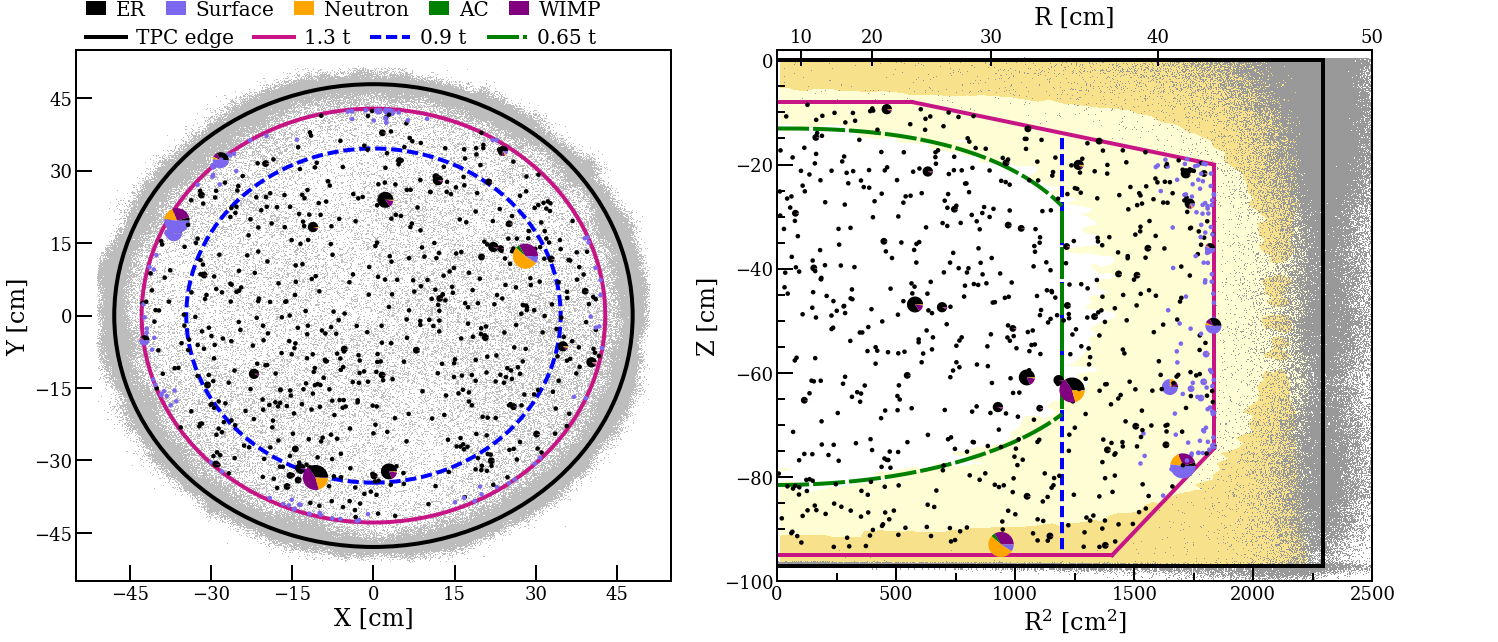
\includegraphics[width=\linewidth]{figures/reconstruction_distribution.png}
	\caption{
	Spatial distribution of dark matter search data.
	The fiducial volume is shown in the magenta and the TPC edge is shown in black.
	Grey points are reconstructed events that are outside the fiducial volume.
	Many of these points are reconstructed outside the bounds of the detector.
	\cite{Xe1T-YearExpo}
	}
	\label{fig:reco-distro}
\end{figure}
\par Using the reconstructed positions, the data from the experiment can be filtered according to the position relative to the fiducial volume.
As shown in Figure \ref{fig:reco-distro}, many of these events are reconstructed near and beyond the wall of the detector.
This can be caused by background events and broken PMTs that will reduce the accuracy of position reconstruction.
Many of these background events are present along the walls due to the radioactivity in the detector's materials \cite{Xe1T-YearExpo}.
However, reconstruction of events outside the detector is clearly not possible for this experiment.
We aim to learn the detector by using a GCNN to minimize these outside reconstructions and minimize the number of reconstructions that are greater than 1 cm away from the true position when applied to simulation.
At the same time, this will be the novel implementation of a GCNN for regression and in particle physics.
\end{document}
